\section*{Introduction}

\begin{frame}{Bibliothèques numériques scientifiques}
    % Il existe plusieurs bibliothèques num sci en fonction des domaines
    % Leur taille croît exponentiellement
    \begin{tikzpicture}
    
        \node (pubmed) {
        
\includegraphics[width=.47\textwidth]{figures/pic_dl/contexte_pubmed.png}
        };
        \node<2>[fill opacity=.85, text opacity=1, fill=white, align=center,text width=2.5cm] at (pubmed) {PubMed \\ Bio-médical \\ 24\,566\,348 doc.};
        
        \node[right=.5cm of pubmed] (arxiv) {
        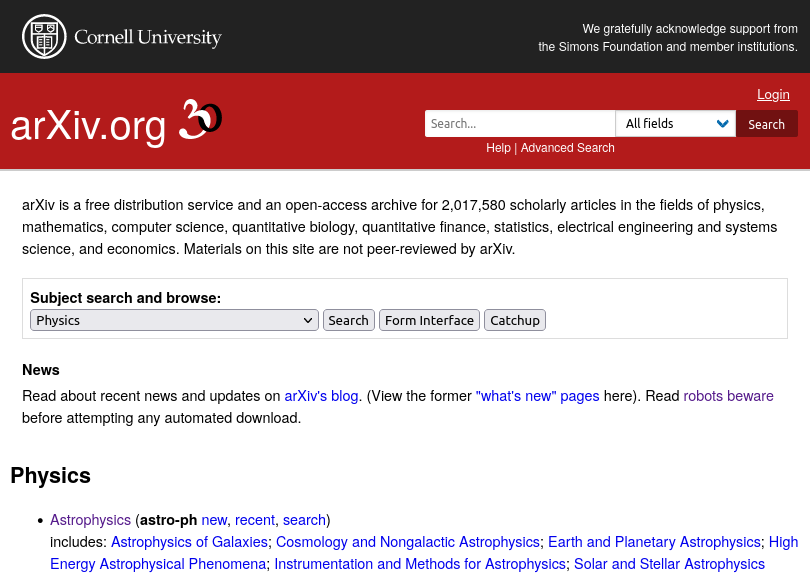
\includegraphics[width=.47\textwidth,trim=0 9em 0 0, clip]{figures/pic_dl/contexte_arxiv.png}
        };
        \node<2>[fill opacity=.75, text opacity=1, fill=white, align=center,text width=3cm] at (arxiv) {arXiv \\ Sciences formelles \\ 1\,999\,642 doc.};
    
        \node[below=.5cm of pubmed] (acmdl) {
        
\includegraphics[width=.47\textwidth]{figures/pic_dl/contexte_acm_dl.png}
        };
        \node<2>[fill opacity=.75, text opacity=1, fill=white, align=center,text width=2.5cm] at (acmdl) {ACMDL\\ Informatique  \\ 654\,532 doc.};
        
        \node[right=.5cm of acmdl] (acl) {
        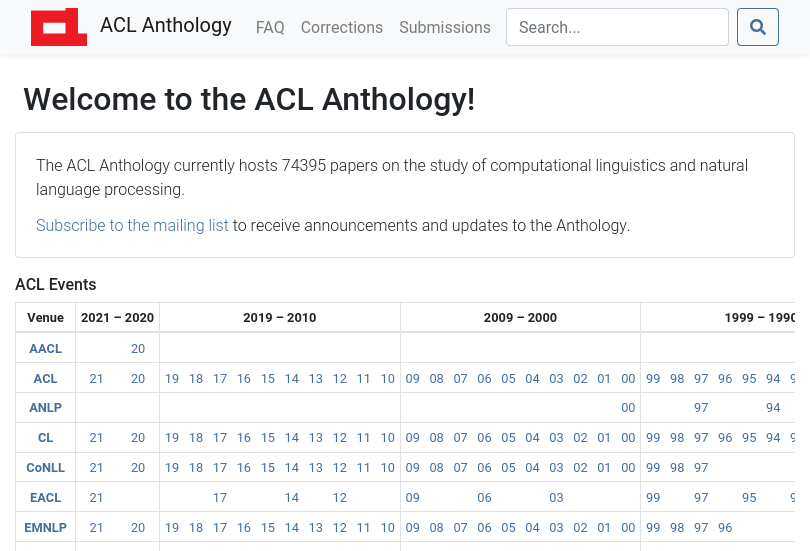
\includegraphics[width=.47\textwidth, trim=0 10em 0 0, clip]{figures/pic_dl/contexte_acl_anthology.png}
        };
        \node<2>[fill opacity=.75, text opacity=1, fill=white, align=center,text width=2.5cm] at (acl) {ACL \\ TALN \\ 74\,432 doc.};
        
        \only<3>{
        \begin{scope}[
            scale=0.4, transform shape]
        \fill[fill opacity=.75, text opacity=1,white] (acmdl.south west) rectangle (acmdl.north east);
        \fill[fill opacity=.75, text opacity=1,white] (pubmed.south west) rectangle (pubmed.north east);
        \fill[fill opacity=.75, text opacity=1,white] (acl.south west) rectangle (acl.north east);
        \fill[fill opacity=.75, text opacity=1,white] (arxiv.south west) rectangle (arxiv.north east);
        
        \pgfplotsset{
            axis x line=bottom, axis y line=left,
            enlargelimits=true,
            xlabel={Année}, ylabel=\text{Soumissions},
            anchor=center,
            x tick label style={ % remove thousands separator for diplaying years https://tex.stackexchange.com/a/31277/240347
                /pgf/number format/.cd, use comma, 1000 sep={},
            },
            every tick label/.append style={font=\Large},
            xtick={2000,2010,2020},
            scaled y ticks=false, % remove scientific notation from axis (https://tex.stackexchange.com/questions/119887/remove-the-scientific-notation-which-is-unreasonable)
        }
        
        \begin{axis}[
            at={(acmdl)},
            ytick={10000,20000,30000},
            yticklabels={10K,20K,30K}]
        \addplot+[smooth] coordinates {
        (1995,6084)(1996,6787)(1997,6942)(1998,7798)(1999,7447)(2000,9096)(2001,8676)(2002,11420)(2003,12994)(2004,15356)(2005,17708)(2006,19777)(2007,20685)(2008,22411)(2009,24403)(2010,27503)(2011,26591)(2012,27302)(2013,26271)(2014,27480)(2015,27498)(2016,28887)(2017,30837)(2018,32890)(2019,35286)(2020,32778)
        %(1995, 43642)(1996, 47134)(1997, 51372)(1998, 50508)(1999, 53524)(2000, 57547)(2001, 57581)(2002, 63690)(2003, 58281)(2004, 66721)(2005, 100763)(2006, 119920)(2007, 120407)(2008, 133729)(2009, 175313)(2010, 146084)(2011, 137865)(2012, 134483)(2013, 112786)(2014, 104140)(2015, 124040)(2016, 117497)(2017, 93819)(2018, 80789)(2019, 81798)(2020, 96451)%(2021, 51069)(2022, 3542)
        };
        \end{axis}
        
        \begin{axis}[
            at={(pubmed)},
            ytick={500000,1000000,1500000},
            yticklabels={{0,5M},1M,{1,5M}}
            ]
        \addplot+[smooth] coordinates {
        (1995, 449050)(1996, 458678)(1997, 456812)(1998, 474666)(1999, 493712)(2000, 532503)(2001, 547504)(2002, 565256)(2003, 594340)(2004, 639530)(2005, 700229)(2006, 749769)(2007, 786530)(2008, 836935)(2009, 877310)(2010, 941684)(2011, 1019685)(2012, 1088548)(2013, 1148929)(2014, 1203202)(2015, 1254639)(2016, 1280910)(2017, 1297742)(2018, 1338381)(2019, 1397240)(2020, 1617944)};
        \end{axis}

        \begin{axis}[
            at={(acl)},
            ytick={2000,4000,6000},
            yticklabels={2K,4K,6K}
            ]
        \addplot+[smooth] coordinates {
        (1995, 386)(1996, 619)(1997, 668)(1998, 1099)(1999, 543)(2000, 1254)(2001, 814)(2002, 1216)(2003, 1186)(2004, 1924)(2005, 1261)(2006, 2149)(2007, 1578)(2008, 2196)(2009, 2204)(2010, 3053)(2011, 2265)(2012, 3375)(2013, 2795)(2014, 3610)(2015, 2945)(2016, 4166)(2017, 3340)(2018, 4597)(2019, 4947)(2020, 7140)%(2021, 6857)
        };
        \end{axis}
        
        \begin{axis}[
            at={(arxiv)},
            ytick={50000,100000,150000},
            yticklabels={50K,100K,150K}]
        \addplot+[smooth] coordinates {
        %(1991, 306)(1992, 3263)(1993, 6743)(1994, 10097)
        (1995, 13014)(1996, 15866)(1997, 19624)(1998, 24172)(1999, 27704)(2000, 30601)(2001, 33214)(2002, 36121)(2003, 39414)(2004, 43727)(2005, 46855)(2006, 50227)(2007, 55638)(2008, 58915)(2009, 64047)(2010, 70131)(2011, 76578)(2012, 84603)(2013, 92641)(2014, 97517)(2015, 105280)(2016, 113380)(2017, 123523)(2018, 140616)(2019, 155866)(2020, 178329)};
        \end{axis}
        \end{scope}
        \node[text width=5cm, align=center] at ($(acmdl)!.5!(arxiv)$) {\textbf{Nombre de soumissions\\par année}};
        }
        
    \end{tikzpicture}
    
\end{frame}

\iffalse
\begin{frame}{Recherche de document}
    % Plus il y a de document, plus c'est difficile de trouver ce que l'on cherche.
    \begin{figure}
        \centering

        \begin{tikzpicture}[spy using outlines={rounded rectangle,magnification=3,width=2cm,height=1cm,connect spies}]
        \node[anchor=south west,inner sep=0] (image) at (0,0) {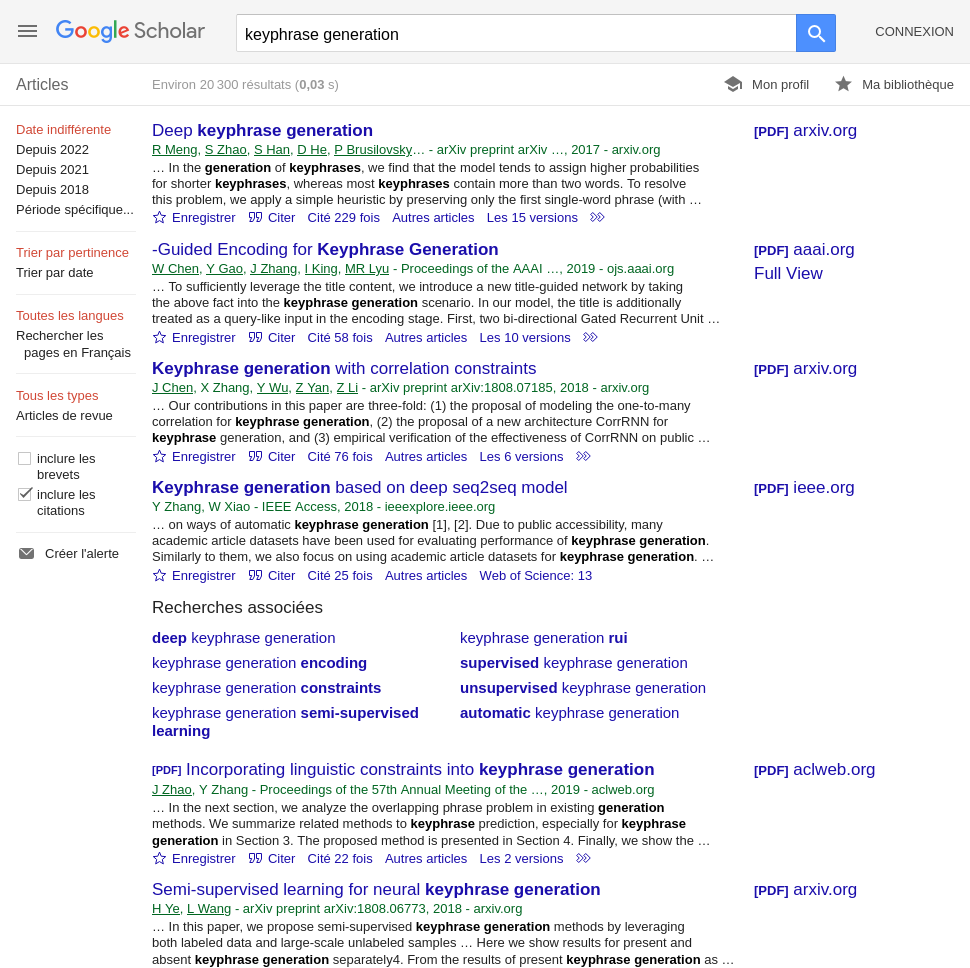
\includegraphics[width=.8\textwidth,trim={0 25em 0 0},clip]{figures/res_dl/google_scholar_all.png}};
        %\draw[help lines,xstep=1,ystep=1] (image.south west) grid (image.north east);
        \spy[blue] on (2, 5.67) in node at (5, 5);
        \end{tikzpicture}
    \end{figure}
\end{frame}
\fi

\begin{frame}{Recherche de document}
    % Plus il y a de document, plus c'est difficile de trouver ce que l'on cherche.
    \begin{figure}
        \centering

        \begin{tikzpicture}[spy using outlines={rounded rectangle,height=1cm}]
        
        \node[anchor=south west,inner sep=0] (image1) at (0,0) {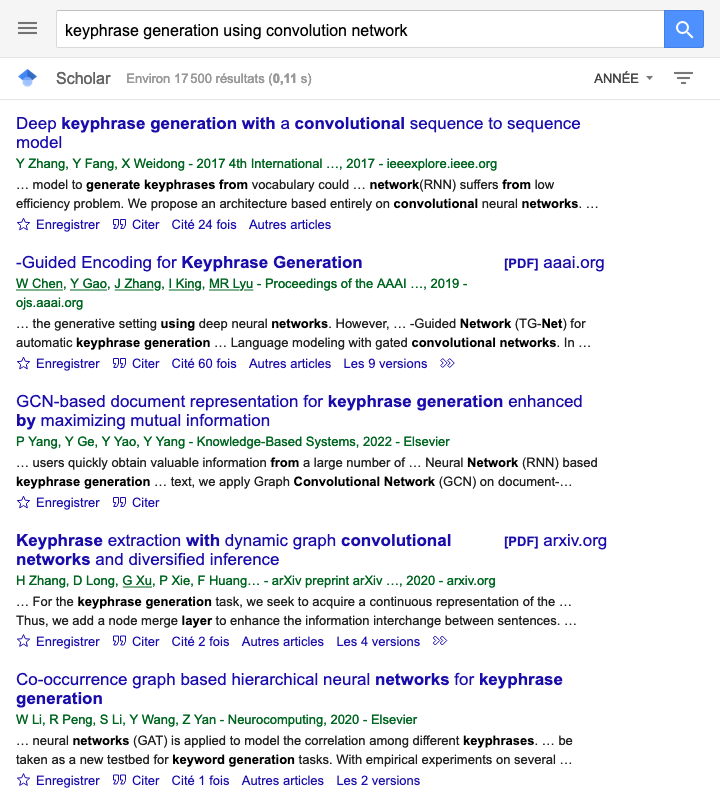
\includegraphics[width=.80\textwidth,,trim=0 30em 0 0,clip]{figures/res_dl/context_scholar-1.png}};
        \spy[blue, magnification=2.25, width=10cm] on (2.9, 5.65) in node at (3.55, 5.8);
        \spy[blue, magnification=3, width=2cm, connect spies] on (2.37, 5.1) in node at (4.5, 5);
        
        %\node[anchor=south west,inner sep=0, right= .25 of image1] (image2) %{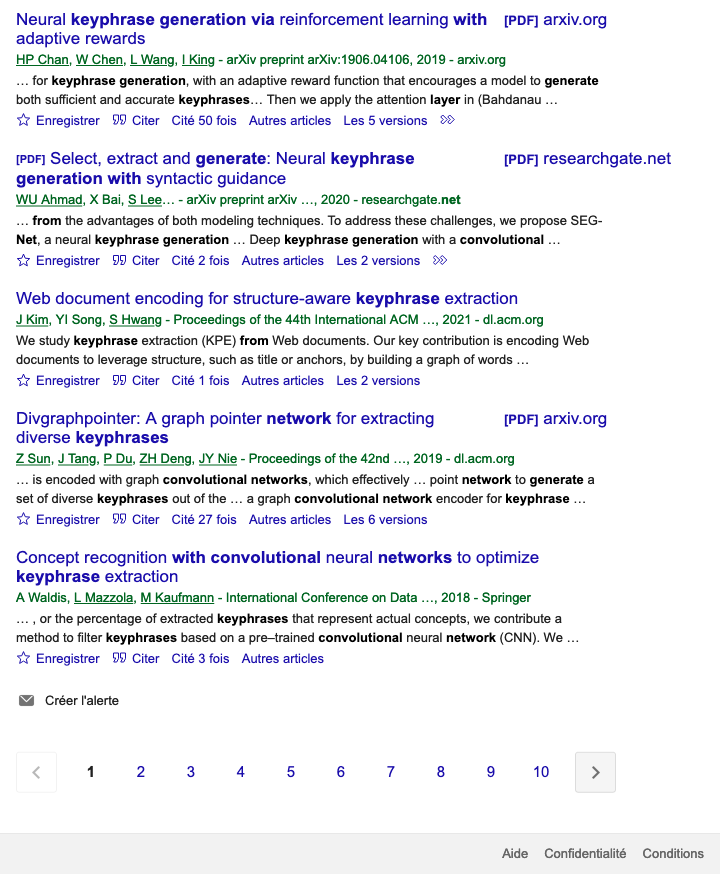
\includegraphics[width=.49\textwidth]{figures/res_dl/context_scholar-2.png}};
        
        %\draw[help lines,xstep=1,ystep=1] (0,0) grid (image1.north east);
        
        %\draw[green, rounded corners] (0.3,5.1) rectangle (4.5,4.2);
        

        \end{tikzpicture}
    \end{figure}
\end{frame}

%\newcommand{\highall}[1]{\textbf<4,5>{\textcolor<4,5>{color0}{#1}}}
%\newcommand{\highkw}[1]{\textbf<4,5>{\textcolor<4,5>{color0}{#1}}}
    
\begin{frame}{Indexation}
    % Indexation: identifier les descripteur d'un document pour pouvoir effectuer une recherche
    % Manuelle: contrôllée (ou non), chère
    % Automatique: grand rappel, petite précision, titre résumé mots-clés
    
    Représenter un document pour qu'il soit facilement recherchable.
    
    
%     \begin{figure}
%     \centering
%     %\centerfloat
%     \resizebox{0.98\textwidth}{!}{%
%     \begin{tabular}{|p{1.3\textwidth}|}
%     \textbf{Recherche d' informations dans un environnement distribué}
%     \vspace{0.9em}
%     Le Web ou les bibliothèques numériques offrent la possibilité d'interroger de nombreux serveurs d' information (collections ou moteurs de recherche) soulevant l'épineux problème de la sélection des meilleures sources de documents et de la fusion des résultats provenant de différents serveurs interrogés. [\ldots]%Dans cet article, nous présentons un nouvelle approche pour la sélection des collections basée sur les arbres de décision. De plus, nous avons évalué différentes stratégies de fusion et de sélection permettant une meilleure vue d'ensemble des différentes solutions.
%     \vspace{1.1em}
%     \textbf{Mots-clés auteur}: recherche d'information, modèle vectoriel, arbre, arbre de décision, moteur de recherche, indexation
%     \vspace{0.2em}
%     \end{tabular}%
%     }
% \end{figure}
    
    \begin{figure}
        \centering
        \begin{annotation}[width=.7\textwidth]{figures/contexte_catalogue_card.jpg}
        %\draw[help lines,xstep=.1,ystep=.1] (0,0) grid (1,1);
        \annoLeft{.8}{Autrice}{.12,.8}
        \annoLeft{.68}{Titre}{.12,.68}
        \annoLeft{.45}{Résumé}{.12,.45}
        \annoLeft{.27}{Sommaire}{.12,.27}
        %\annoLeft{.1}{Mots-clés}{.12,.17}
        \draw[->] (0,.1)++(-\AnnoSep,0) node[anchor=east,onslide={<2>rounded corners, draw=red, thick}]{Mots-clés} -- (.12,.17);
        \end{annotation}
        
        \caption{\scriptsize Notice scientifique. Source: \href{https://www.libraryhistorybuff.org/catalog-cards.htm}{libraryhistorybuff.org/catalog-cards.htm}}
    \end{figure}
    
\end{frame}

\begin{frame}{Indexation par mots-clés}

    Les mots-clés sont généralement des \textbf{syntagmes nominaux} qui représentent les \textbf{concepts les plus importants} d’un document et servent de \textbf{condensateur textuel}.~\cite{amar_les_1997}

    %\azj
    %Leur intérêt principal est d'enrichir l'indexation.

    \begin{block}{Types d'annotation}
        \begin{itemize}
        \item \textbf{indexeur professionnel} (bibliothèque) 
        \item \textbf{auteur} (conférences / journaux)
        \item \textbf{lecteur} (logiciel gestion bibliographique / étudiant·es)
        \end{itemize}
    \end{block}

    \begin{alertblock}{Coût de l'annotation par des indexeurs}
    %\textbf{Coût de l'annotation par des indexeurs} \\
        $\simeq$10\$/doc dans PubMed \\
        \phantom{\textbf{Coût}:} \alt<2>{\textbf{=> 15 M\$ en 2020} et croissance exponentielle !}{}
    \end{alertblock}

\end{frame}


\iffalse
\begin{frame}{Indexation automatique}
    \begin{figure}
        \centering
        %\centerfloat
    \resizebox{0.98\textwidth}{!}{%
    \begin{tabular}{|p{1.3\textwidth}|}
    \color{black!50}
    \highkw{Grammaires} \highall{factorisées} pour des \highkw{dialectes} \highall{apparentés} \\
    \color{black!50}
    Pour la \highall{formalisation} du \highall{lexique} et de la \highkw{grammaire} de \highkw{dialectes} \highall{étroitement apparentés}, il peut se \highall{révéler utile} de \highall{factoriser} une \highall{partie} du \highall{travail} de \highkw{modélisation}. Les \highall{sous systèmes linguistiques} \highall{isomorphes} dans les \highall{différents} \highkw{dialectes} \highall{peuvent} alors faire l'\highall{objet} d'une \highall{\textcolor<5>{color1}{description commune}}, les \highall{différences} étant \highall{spécifiées} par \highall{ailleurs}. Cette \highall{démarche aboutit} à un \highall{modèle} de \highkw{grammaire} à \highall{couches}: le \highall{noyau} est \highall{commun} à la \highall{famille} de \highkw{dialectes}, et une \highall{couche superficielle} \highall{détermine} les \highall{caractéristiques} de \highall{chacun}. Nous \highall{appliquons} ce \highall{procédé} à la \highall{famille} des \highall{langues créoles} à \highall{base lexicale française} de l'\highall{aire américano-caraïbe}.

    \vspace{0.9em}

    \textbf{Mots-clés auteurs}: \highkw{tag, modélisation, grammaire, variation~dialectale}
    \end{tabular}%
    }
    \caption{Notice scientifique du corpus TALN-Archives (id: {\footnotesize taln-2008-long-016})).}
\end{figure}

    \begin{block}{Indexation automatique \say{plein texte}}
    \only<4-5>{
    \begin{itemize}
        \item titre + résumé + mots-clés (auteur / indexeur)
        \item privilégie le rappel
    \end{itemize}
    }
    \end{block}
\end{frame}
\fi

% #1 number of teeths
% #2 radius intern
% #3 radius extern
% #4 angle from start to end of the first arc
% #5 angle to decale the second arc from the first 
\newcommand{\gear}[5]{%
\foreach \i in {1,...,#1} {%
    [rotate=(\i-1)*360/#1]
        (0:#2) arc (0:#4:#2)
        {[rounded corners=1.5pt] -- (#4+#5:#3) arc (#4+#5:360/#1-#5:#3)}
        -- (360/#1:#2)
}}  

\begin{frame}{Production automatique de mots-clés}

    \begin{figure}
    \centering
    \begin{tikzpicture}

    \node[rounded corners, draw=gray!50!black, fill=gray!50, minimum width=1cm, text width=2.5cm, align=center, minimum height=1cm] (method) at (0,0) {Méthode automatique};
    
    \pic[left=2cm of method, local bounding box=doc] {doc={scale 1.5}};
    \node[below=.5cm of doc] {Document};
    
    \pic[right=2cm of method, local bounding box=kws] {kws={scale 1}};
    \node[below=.5cm of kws] {Mots-clés};
    
    \draw[->] (doc.east) -> (method);
    \draw[->] (method) -> (kws.west);

    \end{tikzpicture}
    \end{figure}
    
    \begin{itemize}
        \item 1972: travaux pionniers (\tfidf~\cite{jones_statistical_1972})
        \item 2000: essor des méthodes extractives
        \item 2017: introduction des méthodes génératives
    \end{itemize}
\end{frame}

\begin{frame}{Jeux de données annotés en mots-clés}
    %\newcommand{\tikzmark}[1]{%  \tikz[overlay,remember picture] \node (#1) {};}

%https://tex.stackexchange.com/a/6250/240347
%\alt<3>{\newcolumntype{C}{>{\columncolor{color1!40}}r}}{\newcolumntype{C}{r}}

\begin{table}[htbp!]
\centering
\resizebox{0.8\textwidth}{!}{
    \begin{tabular}{crcccrr}%rr}
    \cmidrule[1pt]{2-7}
        &
        \textbf{Corpus} &
        \textbf{Lang.} &
        \textbf{Ann.} &
        \textbf{\#Entr.} &
        \textbf{\#Test} &
        \textbf{\#mots} \\
        %& \textbf{\#mc} & \textbf{\%abs} \\
    \cmidrule[.5pt]{2-7}
    %\tikzmark{b}
    \rowcolor<2>{color1!40}
    & \cellcolor<3>{color1!40} CSTR~\cite{witten_kea:_1999}              & en & $A$        & \cellcolor<3>{color1!40} 130 & 500 &11501 \\% & 5 & 19 \\
    \rowcolor<2>{color1!40}
    & NUS~\cite{goh_keyphrase_2007}             & en & $A \cup L$ & -   & 211 & 8398 \\% &11 & 14 \\
    \rowcolor<2>{color1!40}
    & PubMed~\cite{schutz_keyphrase_2008}       & en & $A$        & -   & 1320& 5323 \\% & 5 & 17 \\
    \rowcolor<2>{color1!40}
    & ACM~\cite{krapivin_large_2009}            & en & $A$        & -   & 2304& 9198 \\% & 5 & 16 \\
    \rowcolor<2>{color1!40}
    \multirow{-5}{*}[-0.4ex]{\rotatebox{90}{\textbf{Articles}}}
    & Citeulike-180~\cite{medelyan_human-competitive_2009} & en & $L$ & -&182 & 8590 \\% & 5 & 11 \\
    \rowcolor<2>{color1!40}
    & \cellcolor<3>{color1!40} SemEval-2010~\cite{kim_semeval-2010_2010} & en & $A \cup L$ & \cellcolor<3>{color1!40} 144 & 100 & 7961 \\% &15 & 20 \\
    
    %\cmidrule{7-9} %\vspace{-.5em}
    %\multirow{-6}{*}[-0.4ex]{\rotatebox{90}{\textbf{Articles}}}
    %& & & & & \textbf{Avg.} & 8495  & 8  & 16 \\
    
        \cmidrule[.5pt]{2-7}
    
    %\tikzmark{a}
    \rowcolor<2>{color1!40}
    & \cellcolor<3>{color1!40} Inspec~\cite{hulth_improved_2003}         & en & $I$ & \cellcolor<3>{color1!40} 1\,000  & 500    & 135 \\% & 10 & 22 \\
    \rowcolor<2>{color1!40}
    & KDD~\cite{caragea_citation-enhanced_2014} & en & $A$ & -       & 755    & 191 \\% &  4 & 49 \\
    \rowcolor<2>{color1!40}
    & WWW~\cite{caragea_citation-enhanced_2014} & en & $A$ & -       & 1\,330 & 164 \\% &  5 & 52 \\
    \rowcolor<2>{color1!40}
    & TermITH-Eval~\cite{bougouin_termith-eval:_2016} & fr & $I$ & - & 400    & 165 \\% & 12 & 60 \\
    \rowcolor<2>{color1!40}
    \multirow{-5}{*}[-0.4ex]{\rotatebox{90}{\textbf{Notices}}}
    & \cellcolor<3>{color1!60} \textbf<3>{KP20k~\cite{meng_deep_2017}}               & en & $A$ & \cellcolor<3>{color1!60} \textbf<3>{530\,K}  & 20\,K  & 176 \\% &  5 & 43 \\
    %OAGK~\cite{cano_keyphrase_2019-1}         & en & $A$ & 23\,M   & -      & ?   & ?    & ? \\
    %\cmidrule{7-9} %\vspace{-.5em}
    %\multirow{-6}{*}[-0.4ex]{\rotatebox{90}{\textbf{Notices}}}
    %& & & & & \textbf{Avg.} & 166  & 7  & 45 \\
    
    
    \cmidrule[.5pt]{2-7}
    %Reuters-21578~\cite{hulth-megyesi:2006:COLACL}     & en & \\
    %110-PT-BN-KP~\cite{marujo_keyphrase_2011} & pt & $L$ & 100 & 10 & 439 & 27.6 & 7.5 \\
    & DUC-2001~\cite{wan_single_2008}            & en & $L$ & -    & 308 & 847 \\% &  8 &  4 \\
    & \cellcolor<3>{color1!40} 500N-KPCrowd~\cite{marujo_supervised_2012} & en & $L$ & \cellcolor<3>{color1!40} 450  &  50 & 465 \\% & 46 & 11 \\
    \multirow{-4}{*}[-0.4ex]{\rotatebox{90}{\textbf{Journalistique}}}
    & Wikinews~\cite{bougouin_topicrank:_2013}   & fr & $L$ & -    & 100 & 314 \\% & 10 & 11 \\
    %\rowcolor<3>{color1!40}
    %& KPTimes~\cite{gallina_kptimes_2019}        & en & $E$ &\textbf<3>{260\,K}&20\,K& 784 &  5 & 41 \\

    %\cmidrule{7-9} %\vspace{-.5em}
    %\multirow{-5}{*}[-0.4ex]{\rotatebox{90}{\textbf{Journalistique}}}
    %& & & & & \textbf{Avg.} & 603  & 17  & 17 \\
    \cmidrule[1pt]{2-7}
    \end{tabular}
    
    %\tikz[right=5cm,overlay,remember picture] \node[rotate=90, anchor=center] at ($(a)!0.5!(b)$) {Notices};
    %\tikz[overlay,remember picture] \draw[-triangle 45] ($(a.north east)+(-0.2,0.2)$) -- ($(b.south west)+(0.3,-0.2)$);
}
%\caption{\footnotesize Statistiques des jeux de données de production automatique de mots-clés.
%Les mots-clés de référence sont annotés par les auteurs ($A$) ou des indexeurs professionnels ($I$).
%La table présente le nombre de documents dans les corpus d'entraînement (\#Entr.) et de test (\#Test) ainsi que le nombre moyen de mots-clés (\#mc), de mots (\#mots) et le ratio de mots-clés absent (\%abs) par document.}
%\label{tab:datasets_abstract}
\end{table}
    
    \begin{itemize}
        \item Majorité de documents scientifiques
        \item Articles pleins peu accessibles (\emph{paywall})
        
    \end{itemize}
\end{frame}

\begin{frame}<1>[label=problematiques]{Objectifs}
    \begin{enumerate}
        \item \textcolor<2,3>{black!30}{Démontrer la validité des méthodes génératives.}
        \only<1>{
        \begin{itemize}
            \item Entraînement sur plusieurs jeux de données
            \item Généralisation à d'autres genres de documents
        \end{itemize}}
        
        \item \textcolor<1,3>{black!30}{Comparer les performances des méthodes état de l'art.}
        \only<2>{
        \begin{itemize}
            \item Cadre expérimental strict et unifié
            \item Influence du type d'annotation sur l'évaluation
            %\item Influence du type d'annotation sur l'entraînement
        \end{itemize}}
        
        \item \textcolor<1,2>{black!30}{\'Evaluer la qualité des mots-clés au travers d'une tâche applicative.}
        \only<3>{
        \begin{itemize}
            \item Nouveau cadre d'évaluation extrinsèque
            \item Évaluation des méthodes état de l'art
        \end{itemize}}
    \end{enumerate}
    
\end{frame}

\begin{frame}[fragile]{Comparaison des performances}
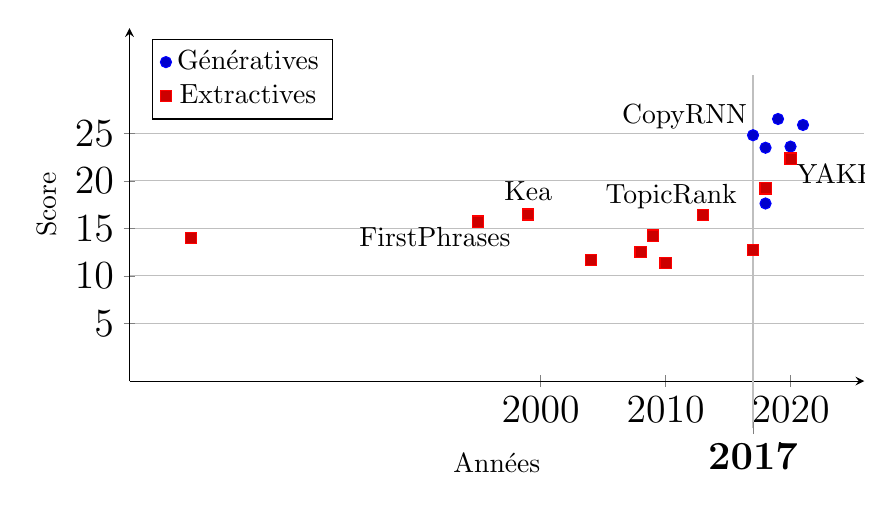
\begin{tikzpicture}
\begin{axis}[
        axis x line=bottom,axis y line = left,enlargelimits=true,
        width=0.9\textwidth,
        height=0.5\textwidth,
        xlabel={Années},
        ylabel={Score},
        ymajorgrids=true,
        ytick={5, 10, 15, 20, 25},
        x tick label style={/pgf/number format/.cd, use comma, 1000 sep={},},
        ymin=2, ymax=33,
        legend pos=north west,
        extra x ticks={2017},
        extra x tick style={grid=major,yshift=-.6cm},
        extra x tick labels={\textbf{2017}}
        ]
\addplot+[only marks] table[meta={end2end}] {
        year mean end2end label
        2017.0 24.82 1 CopyRNN
        2018.0 17.62 1 CorrRNN
        %2018.0 23.76 1 catSeq
        2018.0 23.5 1 catSeqD
        %2019.0 23.52 1 catSeqCorr
        %2019.0 23.98 1 catSeqTG
        2019.0 26.53 1 catSeqTG-2RF1
        2020.0 23.62 1 Transformer
        2021.0 25.9 1 SEG-Net
    };
    \addlegendentry{Génératives}

    \addplot+[only marks] table[meta={end2end}] {
        year mean end2end label
        1972.0 13.96 0 Tf-Idf
        1995.0 15.72 0 FirstPhrases
        1999.0 16.46 0 Kea
        2004.0 11.64 0 TextRank
        %2008.0 10.73 0 ExpandRank
        2008.0 12.49 0 SingleRank
        2009.0 14.24 0 KpMiner
        %2010.0 6.67 0 RAKE
        2010.0 11.34 0 TPR
        2013.0 16.37 0 TopicRank
        2017.0 12.75 0 PositionRank
        2018.0 19.21 0 EmbedRank
        %2018.0 16.57 0 MPRank
        2020.0 22.36 0 YAKE
    };
    \addlegendentry{Extractives}
    \node[inner sep=2pt,anchor=south west] at (axis cs:1972,13.96) {\tfidf};
    \node[inner sep=2pt,anchor=20] at (axis cs:1995,15.72) {FirstPhrases};
    \node[inner sep=2pt,anchor=south east] at (axis cs:2017,24.82) {CopyRNN};
    \node[inner sep=5pt,anchor=south] at (axis cs:1999,16.46) {Kea};
    \node[inner sep=2pt,anchor=north west] at (axis cs:2020,22.36) {YAKE!};
    \node[inner sep=2pt,anchor=330] at (axis cs:2013,16.37) {TopicRank};

\end{axis}
\end{tikzpicture}

Grande diversité de métrique et jeux de données utilisés.

Moyenne des scores rapportés de \textbf{toutes métriques et jeux de données confondus}.

\end{frame}

\begin{frame}[fragile]{Comparaison des performances}
\begin{tikzpicture}
\begin{axis}[
        axis x line=bottom,axis y line = left,enlargelimits=true,
        width=0.9\textwidth, height=0.5\textwidth,
        xlabel={Années}, ylabel={F@5},
        ymajorgrids=true,
        ytick={5, 10, 15, 20, 25},
        x tick label style={/pgf/number format/.cd, use comma, 1000 sep={},},
        ymin=2, ymax=33,
        legend pos=north west,
        extra x ticks={2017},
        extra x tick style={grid=major,yshift=-.6cm},
        extra x tick labels={\textbf{2017}}
        ]
        
    \addlegendimage{mark=*, color=white, fill=color2}
    \addlegendentry{SemEval-2010}
    \addlegendimage{mark=*, color=white, fill=color3}
    \addlegendentry{Inspec}

    \addplot[only marks, mark=*, every mark/.append style={color=white,fill=color2}
    ] table {
        year mean end2end label
        2017 29.23 * CopyRNN
        2018 32.0 * CorrRNN
        2018 24.3 * catSeqD
        2019 28.7 * catSeqTG-2RF1
        2020 25.1 * Transformer
        2021 28.3 * SEG-Net
    };%\addlegendentry{Génératives}
    \addplot[only marks, mark=X*, every mark/.append style={color=white,fill=color2}
    ] table {
        year mean end2end label
        1972 12.8 X* Tf-Idf
        1999 2.5 X* Kea
        2004 17.6 X* TextRank
        2008 13.5 X* SingleRank
        2013 8.3 X* TopicRank
    };%\addlegendentry{SemEval-2010}

    \addplot[only marks, mark=*, every mark/.append style={color=white,fill=color3}
    ] table {
    year mean end2end label
    2017 27.8 * CopyRNN
    2018 22.47 * catSeqD
    2019 25.3 * catSeqTG-2RF1
    2020 21.75 * Transformer
    2021 21.6 * SEG-Net
    };%\addlegendentry{Génératives}
    \addplot[only marks, mark=X*, every mark/.append style={color=white,fill=color3}
    ] table {
    year score end2end method
    1972 22.1 X* Tf-Idf
    2004 22.3 X* TextRank
    2008 21.4 X* SingleRank
    };%\addlegendentry{Inspec}

    \node[inner sep=2pt,anchor=south west] at (axis cs:1972,12.8) {\tfidf};
    %\node[inner sep=2pt,anchor=20] at (axis cs:1995,15.72) {FirstPhrases};
    \node[inner sep=5pt,anchor=east] at (axis cs:2017,29.23) {CopyRNN};
    \node[inner sep=5pt,anchor=south] at (axis cs:1999,2.5) {Kea};
    %\node[inner sep=2pt,anchor=north west] at (axis cs:2020,22.36) {YAKE!};
    \node[inner sep=2pt,anchor=330] at (axis cs:2013,8.3) {TopicRank};

    \draw[dotted] (axis cs:1972,12.8) -- (axis cs:1972,22.1);
    \draw[dotted] (axis cs:2004,17.6) -- (axis cs:2004,22.3);
    \draw[dotted] (axis cs:2008,13.5) -- (axis cs:2008,21.4);
    \draw[dotted] (axis cs:2017,27.8) -- (axis cs:2017,29.23);
    \draw[dotted] (axis cs:2018,24.3) -- (axis cs:2018,22.47);
    \draw[dotted] (axis cs:2019,28.7) -- (axis cs:2019,25.3);
    \draw[dotted] (axis cs:2020,25.1) -- (axis cs:2020,21.75);
    \draw[dotted] (axis cs:2021,28.3) -- (axis cs:2021,21.6);

\end{axis}
\end{tikzpicture}

Score de \textbf{F@5} pour les \textbf{mots-clés présents} sur les jeux de données \textbf{SemEval-2010} et \textbf{Inspec}.

\end{frame}



\againframe<2>{problematiques}


\begin{frame}{\'Evaluation automatique}
    \begin{figure}
    \centering
    \begin{tikzpicture}
    \node (p1) {identité nationale};
    \node[below=.5 of p1] (p2) {pétition en ligne};
    \node[below=.5 of p2] (p3) {france};
    \node[below=.5 of p3] (p4) {internet};
    %\node[below=.5 of p4] (p5) {contestation};
    \node[above=.15 of p1] {\textbf{Référence}};

    \node[draw=green!50!black, rounded corners, fill=green!40, left=of p1, yshift=-.5cm] (r1) {identité nationale};
    %\node[below=.5 of r1] (r2) {forme traditionnelle};
    %\node[below=.5 of r3] (r4) {ligne};
    \node[draw=red!50!black, rounded corners, fill=red!40, below=.5 of r1] (r2) {pétitions électroniques};
    \node[draw=red!50!black, rounded corners, fill=red!40,below=.5 of r2] (r3) {héritières};
    \node[above=.15 of r1, text width=3cm, align=center] {\textbf{Prédiction \\ {\small (TextRank)}}};
    
    \draw[->] (r1) -- (p1);
    \draw[dotted, thick,->] (r2) -- (p2);
    %\draw[loosely dotted, thick,->] (r4) -- (p4);

    %\node[text width=10cm, align=center,below=1.5cm of p4] at ($(r3)!0.5!(p3)$) {\textbf{Titre}: La construction polyphonique des pétitions en ligne:\\Le cas des appels contre le débat sur l'identité nationale. {\footnotesize TermITH-Eval: sciencesInfo\_13-0090563\_tei}};
    \end{tikzpicture}
    \end{figure}
    
    Basée sur l'\textbf{appariement strict} contre une \textbf{référence unique} subjective.
    
    \begin{block}{Métriques}
    Précision; Rappel; F-mesure; MAP
    %P: 1/3; R: 1/4: F: 1/3*1/4 / (1/3+1/4) MAP: (1 + 0 + 0 + 0) / 4
    \end{block}

\end{frame}

\begin{frame}{\'Evaluation automatique}
    \'Evaluation de la \textbf{correspondance} des mots-clés \textbf{à une référence}.
    %\item Quid de la \textbf{qualité} des mots-clés par rapport à leur \textbf{utilisation} dans des tâches aval ?

    \begin{block}{Impact dans les tâches applicatives ?}
    \begin{itemize}
        \item indexation de documents
        %\item détection d'opinion catégorisation de texte, résumé automatique
        \item détection d'opinion%~\cite{berend_opinion_2011}
        \item catégorisation de texte%~\cite{hulth_improved_2003}
        \item résumé automatique%~\cite{zhang_world_2004}
        \item facilitation de la lecture%~\cite{rello_keyword_2014}
    \end{itemize}
    \end{block}
\end{frame}

\againframe<3>{problematiques}